\label{sec:rl_algorithm}

We compared the solutions obtained using the CP and MIP models with those produced by a Q-learning based algorithm.

In Q-learning, an agent learns through repeated interactions with the environment by estimating the action-value function \(Q(s,a)\), which represents the expected \textit{cumulative discounted reward}• obtained by executing action \(a\) in state \(s\) and subsequently following the optimal policy~\cite{watkins1992q}.

After each interaction, the action-value function is updated according to the following rule~\cite{krose1995learning}:

\begin{equation}
	Q(s_t,a_t) \leftarrow Q(s_t,a_t)
	+ \alpha
	\left[
	r_{t+1}
	+ \gamma \max_{a_{t+1}}Q(s_{t+1},a_{t+1})
	- Q(s_t,a_t)
	\right],
	\label{eq:update_q}
\end{equation}

where \(\alpha\) is the learning rate, which determines the influence of newly acquired information on the current estimate, and \(\gamma\) is the discount factor, which balances the importance of immediate and future rewards. In Equation~\eqref{eq:update_q}, the quantity inside the square brackets is the \emph{temporal-difference (TD) error}, which measures the difference between the current estimate and the updated estimate obtained after observing the transition from state \(s_t\) to state \(s_{t+1}\). The term \(r_{t+1}\) denotes the reward obtained after executing action \(a_t\), while \(\max_{a_{t+1}}Q(s_{t+1},a_{t+1})\) represents the estimated value of the best action available in the successor state.

In our formulation, the environment corresponds to the considered workpiece. At each decision step, the state of the environment is defined as

\[
s_t=(n_t,fix_t),
\]

where \(n_t\) is the number of fixtures already placed at step \(t\), while
\(fix_t=[fix_t^{1},\,fix_t^{2},\,\ldots,\,fix_t^{\ntypes}]\)
is an integer array of size \(\ntypes\), whose components denote the remaining availability of the different fixture types.

An action consists of selecting a fixture type together with a feasible centroid position,

\[
a_t=(type_t,(cx_t,cy_t)).
\]

The fixture centroid is used as the reference point for positioning instead of the lower-left corner adopted in the CP and MIP models, since it simplifies both the enforcement of the horizontal and vertical safety-distance constraints, as described in Section~\ref{sec:cp_cons}, and the identification of feasible actions.

The action to be executed is selected according to an \textit{\(\epsilon\)-greedy policy}~\cite{sutton1998reinforcement}. At each decision step, the agent selects the action with the highest estimated \(Q\)-value with probability \(1-\epsilon\), whereas with probability \(\epsilon\) it selects a random action, balancing exploration and exploitation of the environment.

The Q-learning based procedure adopted for fixture layout optimization is described in Algorithm~\ref{alg:qlearning_fixtures}. The algorithm takes as inputs the number of training episodes \(E\), the maximum number of steps per episode \(T\), the learning rate \(\alpha\), the discount factor \(\gamma\), the exploration rate \(\epsilon\), and the exploration decay factor \(\rho\). The output is the best feasible fixture layout \(\mathcal{L}^{*}\) obtained by applying the learned policy.

\begin{algorithm}[t]
	\footnotesize
	\caption{Q-learning for Fixture Layout Optimization}
	\label{alg:qlearning_fixtures}
	\begin{algorithmic}[1]
		
		\Require Number of episodes $E$, maximum number of steps per episode $T$, learning rate $\alpha$, discount factor $\gamma$, exploration rate $\epsilon$, exploration decay factor $\rho$
		\Ensure Best feasible layout $\mathcal{L}^*$
		
		\State Compute all candidate centroid positions
		\label{alg:q_init_start}
		\State Remove centroid positions violating the constraints and set $\mathcal{A}(s_1)$
		\State Initialize $Q(s,a)=0$
		\State $\mathcal{L}^* \gets \emptyset$
		\label{alg:q_init_end}
		
		\For{$ep=1$ to $E$}
		\label{alg:q_iteration_start}
		
		\For{$t=1$ to $T$}
		
		% \State Compute the feasible action set $\mathcal{A}(s_t)$
		
		\If{$\mathcal{A}(s_t)=\emptyset$}
		\State \textbf{break}
		\EndIf
		\label{alg:q_iteration_end}
		
		\If{random number $<\epsilon$} \Comment{exploration}
		\label{alg:q_policy_start}
		\State Select a random feasible action
		$a_t \in \mathcal{A}(s_t)$
		\Else \Comment{exploitation}
		\State Select
		$a_t=\arg\max\limits_{a\in\mathcal{A}(s_t)}Q(s_t,a)$
		\EndIf
		
		\State Perform action $a_t$ by placing the selected fixture
		\label{alg:q_policy_end}
		
		\State Recompute the feasible action set $\mathcal{A}(s_{t+1})$ 
		\label{alg:q_reset_action}
		
		\State Compute reward $r_t$ according to Eq.~\ref{eq:reward}
		\label{alg:q_update_start}
		
		\State Observe successor state $s_{t+1}$
		
		\State $Q(s_t,a_t) \gets Q(s_t,a_t) + \alpha \left[r_{t+1} + \gamma \max_{a_{t+1}}Q(s_{t+1},a_{t+1}) - Q(s_t,a_t) \right]$
		
		\State $s_t \gets s_{t+1}$
		\State Update $\mathcal{L}_{ep}$ with $a_t$
		\label{alg:q_update_end}
		
		\EndFor
		
		\If{$\mathcal{L}_{ep}$ is better than $\mathcal{L}^*$}
		\State $\mathcal{L}^* \gets \mathcal{L}_{ep}$
		\EndIf
		\State $\epsilon \gets \rho\,\epsilon$
		\State Reset the environment to the initial state $s_1$
		\State Reset the action space to $\mathcal{A}(s_1)$
		
		\EndFor
		
		\State Evaluate the learned policy using greedy action selection
		\label{alg:q_evaluate_start}
		\State \textbf{return} $\mathcal{L}^*$
		\label{alg:q_evaluate_end}
		
	\end{algorithmic}
\end{algorithm}

Given the fixture dimensions, it is known \emph{a priori} that some positions within the workpiece cannot accommodate a fixture, particularly those near the workpiece boundary or close to areas to be extruded. During the initialization phase, in lines~\ref{alg:q_init_start}--\ref{alg:q_init_end} of Algorithm~\ref{alg:qlearning_fixtures}, centroid positions that would result in fixtures extending outside the workpiece boundaries or overlapping extrusion areas are removed from the set of possible actions \(\mathcal{A}(s_t)\), considering the dimensions of the smallest fixture as reference.

Figure~\ref{fig:q_learning_actions} shows an example of the set of feasible actions for a given workpiece, considering two available fixture types: square and rectangular. Green dots indicate centroid positions where both fixture types can be placed, whereas red dots indicate positions where only rectangular fixtures can be placed.

The algorithm iterates over the training episodes and the corresponding steps. An episode terminates when no feasible actions remain or the maximum number of steps is reached, as shown in lines~\ref{alg:q_iteration_start}--\ref{alg:q_iteration_end} of Algorithm~\ref{alg:qlearning_fixtures}.

The agent selects actions according to the \(\epsilon\)-greedy policy (lines~\ref{alg:q_policy_start}--\ref{alg:q_policy_end} of Algorithm~\ref{alg:qlearning_fixtures}), balancing the exploration of new placements with the exploitation of previously learned actions.

Each action selected is evaluated through the reward associated with the transition from \(s_t\) to \(s_{t+1}\). The reward function combines the improvement obtained in the moment of inertia with additional terms promoting layouts composed of a larger number of fixtures, larger fixture dimensions, and increased spatial separation between fixtures:

\begin{equation}
	r_{t+1}
	=
	\lambda_{\mathrm{iner}}\,\Delta\finer
	+
	\lambda_n n_{t+1}^{2}
	+
	\lambda_d\bar d
	+
	\begin{cases}
		b_{\nmin}, & \text{if } n_{t+1}\geq\nmin,\\
		0, & \text{otherwise}.
	\end{cases}
	\label{eq:reward}
\end{equation}

In the equation: 
\begin{itemize} 
	\item $\Delta\finer$ is the variation of $\finer$ between the previous and current states;
	\item \(n_{t+1}\) is the number of fixtures in the resulting layout. The quadratic term promotes layouts with a larger number of fixtures;
	\item \(\bar d\) is the average Euclidean distance between the newly placed fixture and the previously placed fixtures,  promoting layouts with a larger spatial separation;
	\item \(\lambda_{\finer}\), \(\lambda_n\), and \(\lambda_d\) are weighting coefficients balancing the contribution of the different reward components;
	\item \(b_{\nmin}\) is an additional feasibility bonus assigned when the minimum required number of fixtures, \(\nmin\), has been placed.
\end{itemize}

After each fixture placement, all candidate centroid positions that no longer satisfy the safety-distance constraints are removed from the feasible action set, as shown in line~\ref{alg:q_reset_action} of Algorithm~\ref{alg:qlearning_fixtures}. Consequently, the action set progressively shrinks as the layout is constructed, ensuring that all geometric constraints are satisfied.

The only constraint that cannot be enforced by restricting the feasible action set is the placement of the minimum number of required fixtures \(\nmin\). For this reason, the feasibility bonus \(b_{\nmin}\) is included in the reward function to encourage the agent to generate layouts satisfying this constraint.

After executing the selected action, the corresponding reward is computed, the \(Q\)-function value associated with state \(s_t\) and action \(a_t\) is evaluated and the learned policy is updated (lines~\ref{alg:q_update_start}--\ref{alg:q_update_end} of Algorithm~\ref{alg:qlearning_fixtures}).

Finally, after all training episodes have been completed, the learned policy is evaluated to obtain the fixture layout for the considered workpiece, as shown in lines~\ref{alg:q_evaluate_start}--\ref{alg:q_evaluate_end} of Algorithm~\ref{alg:qlearning_fixtures}.

\begin{figure}[t]
	\centering
	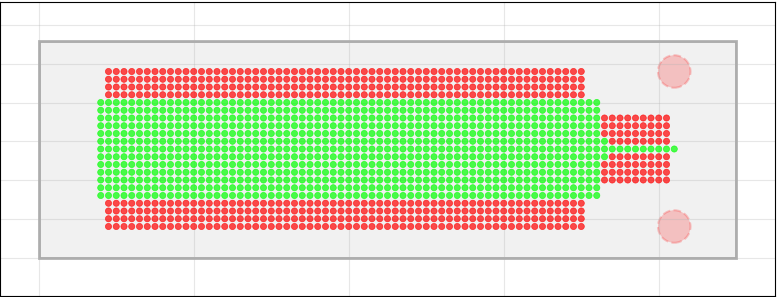
\includegraphics[width=0.5\linewidth]{img/q_learning_actions.png}
	\caption{Example of the available actions for a given workpiece. Green dots represent centroid positions where both square and rectangular fixtures can be placed, whereas red dots represent positions where only rectangular fixtures can be placed. The workpiece area is highlighted in light gray, while the areas to be extruded are highlighted in red.}
	\label{fig:q_learning_actions}
\end{figure}
